\subsection{Organització de l'equip}
\label{metodologia:oranitzacio_equip}
Al tractar-se d'un projecte realitzat en una empresa, conjuntament amb l'equip de desenvolupadors d'aquesta, el més normal és que s'adopti la manera de funcionar i organitzar-se de l'equip.\\
En aquest cas concret, la forma d'organització és mitjançant \textit{Scrum}.\\
\newline \textit{Scrum} és, de les conegudes com ``metodologies àgils'' la de més renom i provada eficàcia. Alhora, donada la tipologia de l'equip, sovint es fa ús de la coneguda com \textit{Kanban}, però sense oblidar les bondats d'\textit{scrum}.\\
\newline Per una banda, \textit{scrum} planteja un funcionament a base d'iteracions (\textit{sprints}) generalment de dues o quatre setmanes on al principi de cada una d'aquestes iteracions es manté una reunió (\textit{Sprint Planning Meeting}) on es busca planificar les tasques a desenvolupar al llarg de l'\textit{sprint} que comença el mateix dia de la reunió.
\begin{figure}[h]
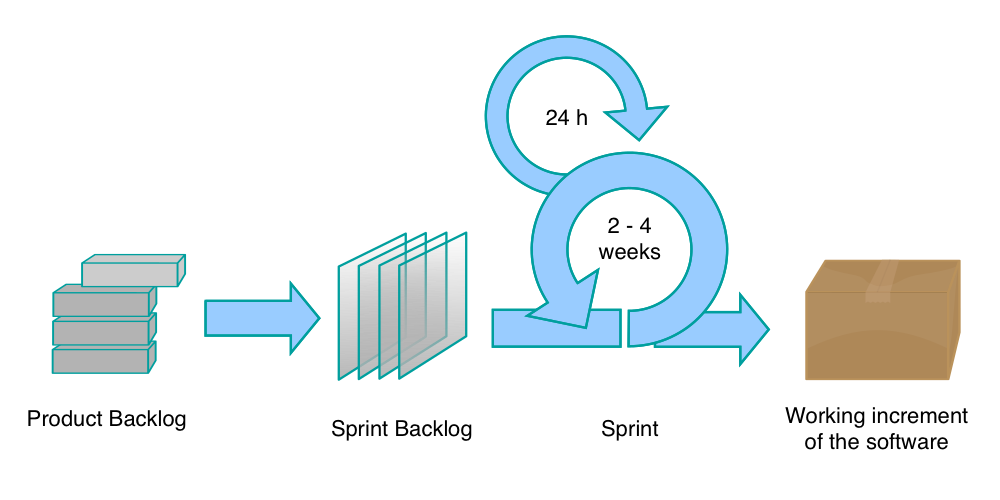
\includegraphics[scale=0.4]{sections/gestio/scrum_process.png}
\centering
\caption{Scrum}
\label{fig:scrum}
\end{figure}
\newline De la mateixa manera, \textit{scrum} proposa un seguit de reunions diàries on cada un dels membres de l'equip ha de respondre les següents preguntes:
\begin{itemize}
	\item Què es va fer ahir?
	\item Què es farà avui?
	\item Quins impediments s'han trobat fins ara?
\end{itemize}
El simple fet de respondre les anteriors preguntes, dóna als membres de l'equip una visió global de l'estat actual del projecte i permet intentar buscar solucions als entrebancs que puguin sorgir d'una forma col·laborativa on cada desenvolupador pot aportar el seu punt de vista i possibles solucions.\\
\newline Alhora, aquestes reunions permeten identificar desviacions del projecte i trobar-hi la solució adient abans de que el problema afecti de forma real, al global del projecte.\\
\newline \textit{Kanban} pel seu costat planteja l'acumulació de totes les tasques a desenvolupar en un mateix \textit{dashboard} visible per a tots els membres de l'equip organitzat en tres columnes:
\begin{itemize}
    \item \textit{ToDo}: on s'acumulen totes les tasques en el realitzar al projecte.
    \item \textit{Doing}: passen a aquesta columna només les que cada desenvolupador està realitzant en aquell moment.
    \item \textit{Done}: on s'acumulen les tasques ja finalitzades.
\end{itemize}
A mesura que avança el projecte, la idea és que cada desenvolupador agafi tasques de la columna \textit{ToDo} i les vagi passant a la columna \textit{Done}.\\
\newline Així doncs, en el cas concret d'aquest projecte, la dinàmica de l'equip ha estat la de fer ús de \textit{kanban} i el seu \textit{dashboard} de tres columnes, sense renunciar a la bondat de les \textit{daylies} que proposa \textit{scrum}.\\
\newline Aquesta barreja de metodologies ha permès detectar problemes i solucionar-los a temps, tal i com es veurà posteriorment al llarg de la secció \namref{desenvolupament}.
%Per al desenvolupament del projecte s'adoptaran les metodologies emprades a l'empresa, que en aquest cas, són el que s'anomenen metodologies àgils; concretament l'anomenada \textit{Scrum}\cite{scrum}.\\
%\\\textit{Scrum} es basa en la realització d'iteracions durant el procés de desenvolupament que reven el nom d'\textit{sprints}. Les esmentades iteracions es composen d'un seguit de tasques que s'han de completar al llarg de la durada dels \textit{sprints}; que acostuma a oscil·lar entre una setmana i un mes.\\
%\\Els objectius a assolir durant l'\textit{sprint} es fixen en unes reunions que es duen a terme a l'inici anomenades \textit{Sprint Planning Meeting}.\\
%Per altra banda, durant l'exercici de l'\textit{sprint} es realitzen reunions periòdiques anomenades \textit{Daily Scrum Meetings}, on es tracta de respondre a les següents preguntes:
%\begin{itemize}
%	\item Què es va fer ahir?
%	\item Què es farà avui?
%	\item Quins impediments s'han trobat fins ara?
%\end{itemize}
%Les anteriors preguntes intenten donar una visió el més àmplia possible de l'estat del projecte a tots els memebres de l'equip, així com permetre la resolució col·laborativa dels diferents problemes que vagin apareixent al llarg del desenvolupament.\\
%\\\textit{Scrum} permet reaccionar de forma àgil a les diferents alteracions que poden sorgir al llarg del desenvolupament i que els desenvolupadors realitzin els canvis pertinents.\\
%\\Al tractar-se d'un equip de desenvolupament reduït on la comunicació entre membres és constant, el seguiment de la filosofia \textit{scrum} resulta a vegadas un tant òbvia. Tot i aixó, es respecten les \textit{daylies} a l'inici de cada jornada i els \textit{sprint plannings} a l'inici de cada iteració.